\renewcommand{\thesection}{\arabic{section}}\renewcommand{\theHsection}{chapter.\arabic{section}}\setcounter{section}{2}\section{函数的导数}
\noindent\begin{minipage}{\textwidth}\ProblemHeading{例题}{3.1（改写）}
一质点作非匀速直线运动，其位置与时间的关系为 $s=s(t)$。写出时间段 $[t,t+\Delta t]$ 上的平均速度，并用极限给出时刻 $t$ 的瞬时速度；说明所需的极限存在条件。
\end{minipage}\par\vfill
\noindent\begin{minipage}{\textwidth}\ProblemHeading{例题}{3.2（改写）}
一根非均匀细棒的横截面处处相同。设从左端 $A$ 到距 $A$ 为 $x$ 处的一段细棒质量为 $m(x)$。写出从 $x$ 到 $x+\Delta x$ 这一段的平均线密度，并用极限定义 $x$ 处的线密度，说明所需条件。
\end{minipage}\par\vfill
\noindent\begin{minipage}{\textwidth}\ProblemHeading{例题}{3.3（改写）}
曲线 $y=f(x)$ 上有定点 $P_0=(x_0,f(x_0))$ 和动点 $P=(x,f(x))$。写出割线 $P_0P$ 的斜率，并在该斜率随 $x\to x_0$ 有有限极限时，求曲线在 $P_0$ 处的切线方程。
\end{minipage}\par\vfill
\newpage
\noindent\begin{minipage}{\textwidth}\ProblemHeading{例题}{3.4}
设 $f(x)=|x|$。证明 $f$ 在 $x=0$ 处不可导。
\end{minipage}\par\vfill
\noindent\begin{minipage}{\textwidth}\ProblemHeading{习题}{3.5}
设 $f$ 在 $0$ 处可导且 $f(0)=0$。求 $\lim_{x\to0}f(x)/x$。
\end{minipage}\par\vfill
\noindent\begin{minipage}{\textwidth}\ProblemHeading{习题}{3.6}
设 $f$ 在 $0$ 处可导，$a_n\to0^-$、$b_n\to0^+$。证明 $\lim_{n\to\infty}\dfrac{f(b_n)-f(a_n)}{b_n-a_n}=f^{\prime}(0)$。
\end{minipage}\par\vfill
\newpage
\noindent\begin{minipage}{\textwidth}\ProblemHeading{习题}{3.7}
设 $f$ 为偶函数且在 $0$ 处可导。证明 $f^{\prime}(0)=0$。
\end{minipage}\par\vfill
\noindent\begin{minipage}{\textwidth}\ProblemHeading{习题}{3.8}
设 $f$ 在 $x_0$ 处可导。证明 $\lim_{h\to0}\dfrac{f(x_0+h)-f(x_0-h)}{2h}=f^{\prime}(x_0)$；再举例说明，即使左边的极限存在且有限，$f$ 在 $x_0$ 也未必可导。
\end{minipage}\par\vfill
\noindent\begin{minipage}{\textwidth}\ProblemHeading{习题}{3.9}
在抛物线 $y=x^2$ 上求满足下列条件的点：
\SubQ{1}{切线平行于直线 $y=4x-5$。}
\SubQ{2}{切线垂直于直线 $2x-6y+5=0$。}
\SubQ{3}{切线与直线 $3x-y+1=0$ 成 $45^\circ$ 角。}
\end{minipage}\par\vfill
\newpage
\noindent\begin{minipage}{\textwidth}\ProblemHeading{习题}{3.10}
证明抛物线 $y=x^2$ 在 $(x_1,x_1^2)$、$(x_2,x_2^2)$ 处的切线互相垂直，当且仅当 $4x_1x_2+1=0$。
\end{minipage}\par\vfill
\noindent\begin{minipage}{\textwidth}\ProblemHeading{习题}{3.11}
设 $f$ 在 $a$ 处可导且 $f(a)\ne0$。求 $\lim_{n\to\infty}\left(\dfrac{f(a+1/n)}{f(a)}\right)^n$。
\end{minipage}\par\vfill
\noindent\begin{minipage}{\textwidth}\ProblemHeading{习题}{3.12}
设 $\varphi$ 在 $a$ 处连续，并在 $a$ 附近定义 $f(x)=(x-a)\varphi(x)$、$g(x)=|x-a|\varphi(x)$。证明 $f$ 在 $a$ 处可导并求 $f^{\prime}(a)$；求 $g$ 在 $a$ 处可导的充要条件。
\end{minipage}\par\vfill
\newpage
\noindent\begin{minipage}{\textwidth}\ProblemHeading{习题}{3.13}
设 $f(x)=x(x-1)^2(x-2)^3$。求 $f^{\prime}(0)$、$f^{\prime}(1)$、$f^{\prime}(2)$。
\end{minipage}\par\vfill
\noindent\begin{minipage}{\textwidth}\ProblemHeading{习题}{3.14（校订）}
设 $\lambda\in\mathbb R$，$f(0)=0$，$f(x)=|x|^\lambda\sin(1/x)$（$x\ne0$）。证明：$\lambda>1$ 时 $f^{\prime}(0)$ 存在，$\lambda\le1$ 时 $f$ 在 $0$ 处不可导。
\end{minipage}\par\vfill
\noindent\begin{minipage}{\textwidth}\ProblemHeading{习题}{3.15}
定义 Riemann 函数 $R(x)=1/q$，当 $x=p/q\in\mathbb Q$ 为既约分数且 $q>0$；对无理数令 $R(x)=0$。证明 $R$ 处处不可导。
\end{minipage}\par\vfill
\newpage
\noindent\begin{minipage}{\textwidth}\ProblemHeading{习题}{3.16}
构造一个在 $\mathbb R$ 上处处不可导的函数 $f$，使得对每个实数 $x$，$\lim_{n\to\infty}n\bigl(f(x+1/n)-f(x)\bigr)$ 都存在。
\end{minipage}\par\vfill
\noindent\begin{minipage}{\textwidth}\ProblemHeading{例题}{3.17}
用导数定义证明常值函数 $f(x)=c$ 的导数恒为 $0$。
\end{minipage}\par\vfill
\noindent\begin{minipage}{\textwidth}\ProblemHeading{例题}{3.18}
用导数定义计算 $f(x)=x^n$（$n\in\mathbb N^*$）的导数。
\end{minipage}\par\vfill
\newpage
\noindent\begin{minipage}{\textwidth}\ProblemHeading{例题}{3.19}
用导数定义求 $f(x)=x^\alpha$（$x>0$，$\alpha\in\mathbb R$）的导数。
\end{minipage}\par\vfill
\noindent\begin{minipage}{\textwidth}\ProblemHeading{例题}{3.20}
用导数定义求正弦函数 $f(x)=\sin x$ 的导数。
\end{minipage}\par\vfill
\noindent\begin{minipage}{\textwidth}\ProblemHeading{例题}{3.21}
用导数定义证明 $(\cos x)^{\prime}=-\sin x$。
\end{minipage}\par\vfill
\newpage
\noindent\begin{minipage}{\textwidth}\ProblemHeading{例题}{3.22}
设 $a>0$。求 $f(x)=a^x$ 的导数。
\end{minipage}\par\vfill
\noindent\begin{minipage}{\textwidth}\ProblemHeading{例题}{3.23}
求正切函数 $\tan x$ 与余切函数 $\cot x$ 在各自定义域内的导数。
\end{minipage}\par\vfill
\noindent\begin{minipage}{\textwidth}\ProblemHeading{例题}{3.24}
设 $y=\cos(x^2+5x+2)$。求 $y^{\prime}$。
\end{minipage}\par\vfill
\newpage
\noindent\begin{minipage}{\textwidth}\ProblemHeading{例题}{3.25}
设 $y=\sin\ln\dfrac{x}{1+x^2}$（$x>0$）。求 $y^{\prime}$。
\end{minipage}\par\vfill
\noindent\begin{minipage}{\textwidth}\ProblemHeading{例题}{3.26}
求 $y=\ln\bigl(x+\sqrt{a^2+x^2}\bigr)$ 的导数，其中 $a$ 为常数，在函数有定义且可导的范围讨论。
\end{minipage}\par\vfill
\noindent\begin{minipage}{\textwidth}\ProblemHeading{例题}{3.27（校订）}
求 $y=\log_a x$（$a>0$，$a\ne1$，$x>0$）的导数。
\end{minipage}\par\vfill
\newpage
\noindent\begin{minipage}{\textwidth}\ProblemHeading{例题}{3.28}
计算下列反三角函数的导数：
\SubQ{1}{$f(x)=\arcsin x$。}
\SubQ{2}{$f(x)=\arctan x$。}
\end{minipage}\par\vfill
\noindent\begin{minipage}{\textwidth}\ProblemHeading{例题}{3.29（改写）}
设 $u,v$ 可导且 $u(x)>0$。求幂指函数 $f(x)=u(x)^{v(x)}$ 的导数。
\end{minipage}\par\vfill
\noindent\begin{minipage}{\textwidth}\ProblemHeading{例题}{3.30（改写）}
设 $f$ 为恒正的可导函数。证明对数求导公式 $f^{\prime}(x)=f(x)(\ln f(x))^{\prime}$，并用它求 $f(x)=u_1(x)\cdots u_n(x)$ 的导数，其中各 $u_i$ 均为正的可导函数。
\end{minipage}\par\vfill
\newpage
\noindent\begin{minipage}{\textwidth}\ProblemHeading{例题}{3.31}
一正圆锥容器底面水平、顶点在上，底半径为 $R\,\mathrm{cm}$，顶点有小孔供注水。以恒定体积速率 $A\,\mathrm{cm}^3/\mathrm{s}$ 注水，求水位达到锥高一半时水面上升的速度（$R,A>0$）。
\begin{center}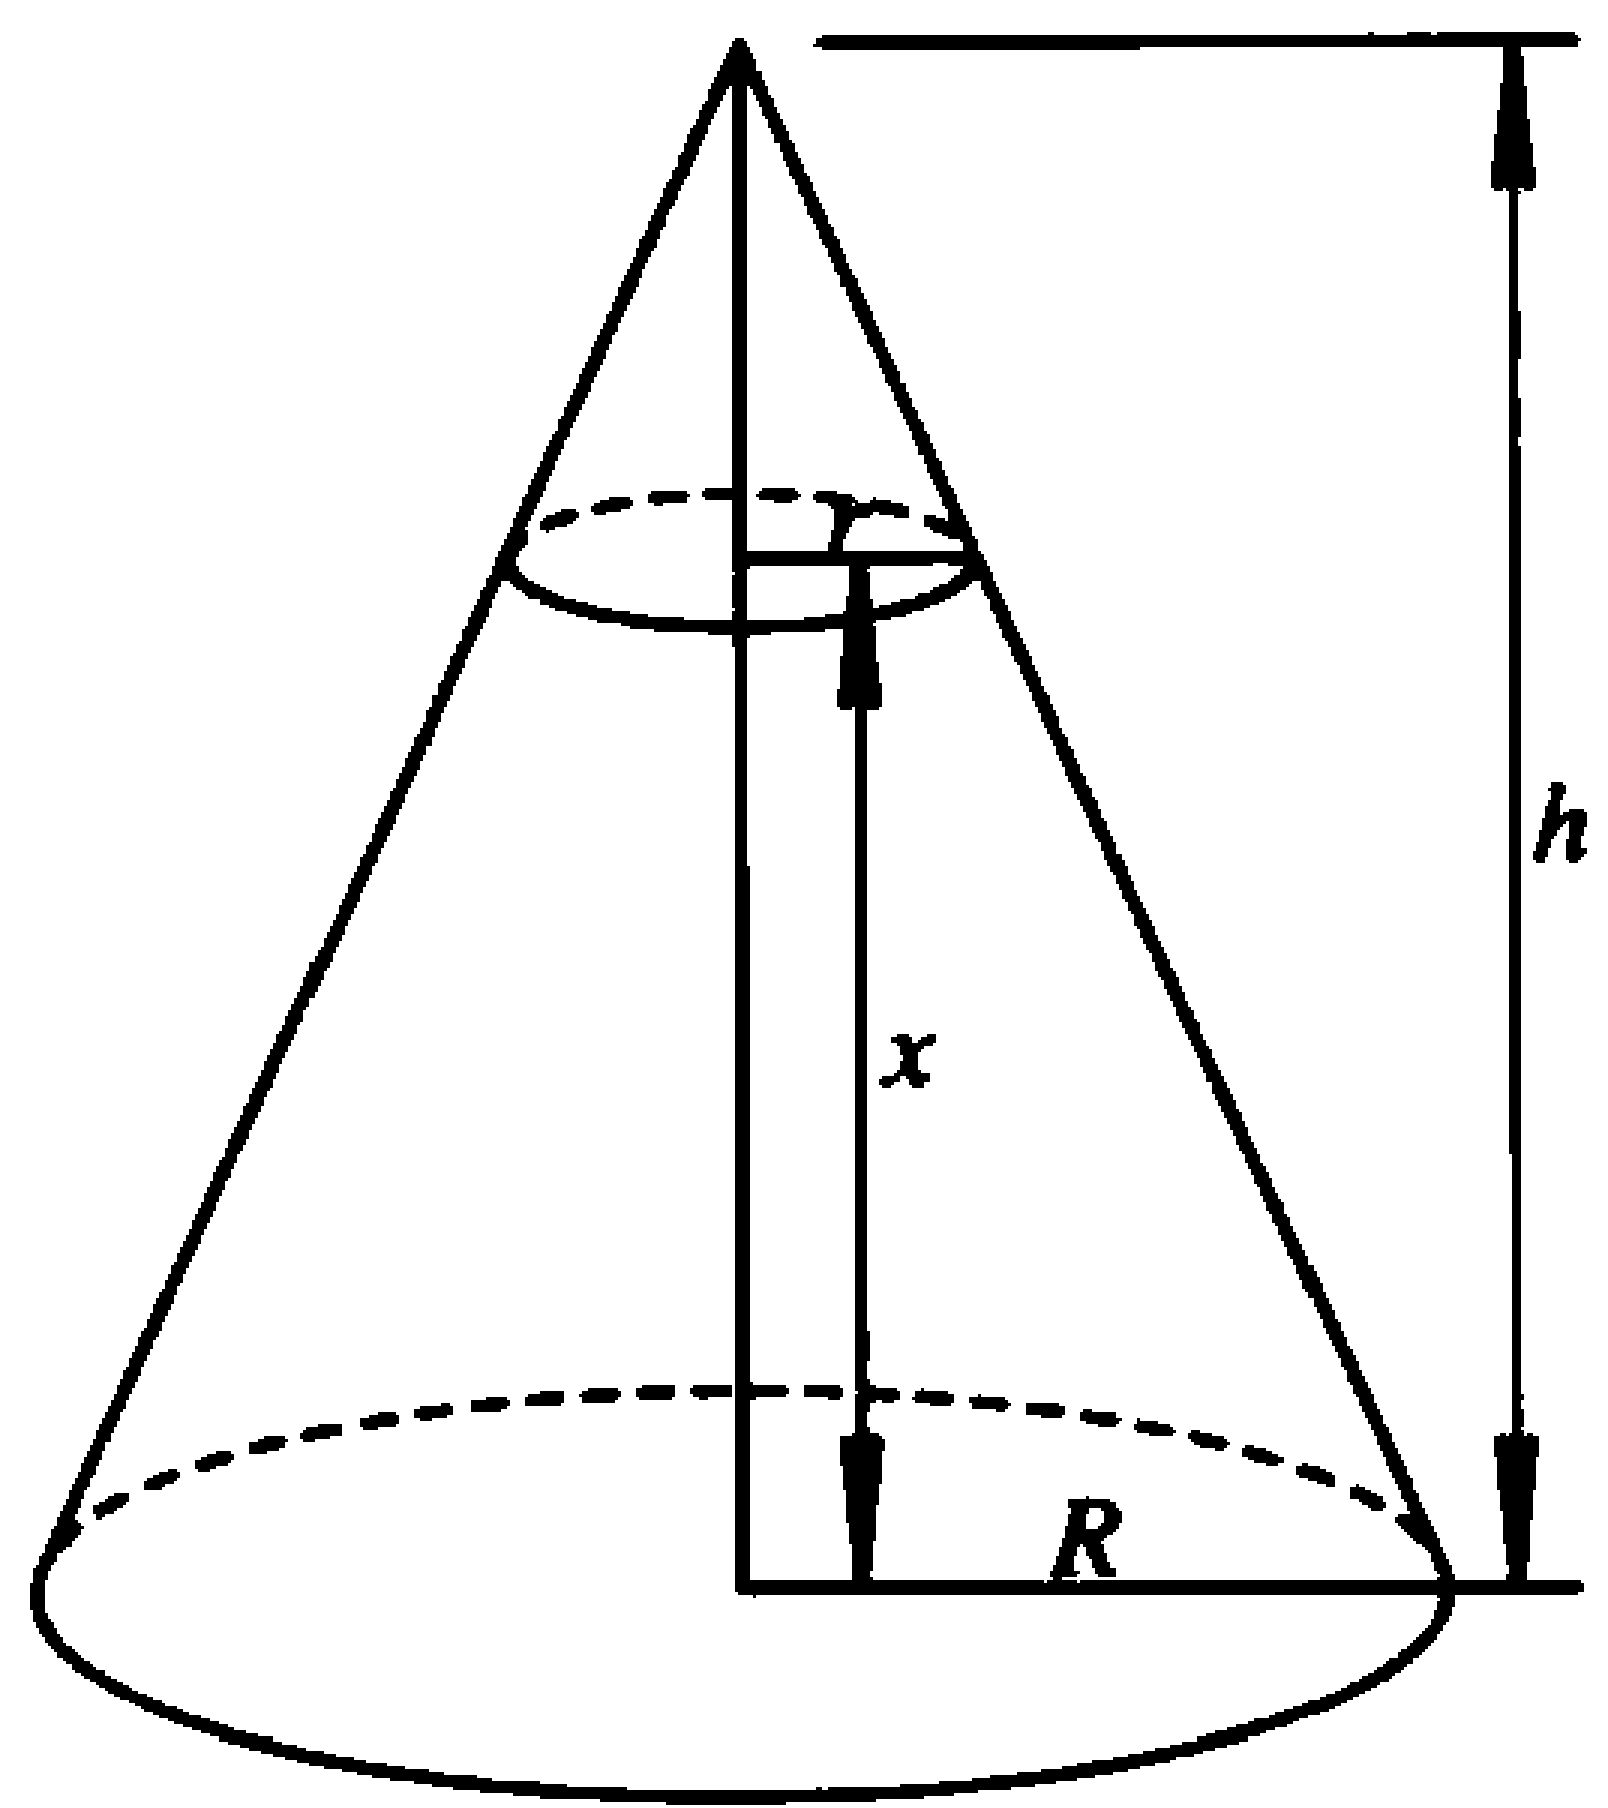
\includegraphics[width=0.31\linewidth]{figures/fig_3_31_1.png}\end{center}
\end{minipage}\par\vfill
\newpage
\noindent\begin{minipage}{\textwidth}\ProblemHeading{习题}{3.32（校订）}
求下列函数的导数；出现的 $a,b,c,d$ 均为常数，按自然定义域讨论：
\SubQ{1}{$y=x^3-2x+6$。}
\SubQ{2}{$y=\sqrt{x}-1/x$。}
\SubQ{3}{$y=a\cos x+b\sin x$。}
\end{minipage}\par\vfill
\noindent\begin{minipage}{\textwidth}\ProblemHeading{习题}{3.33（校订）}
求下列函数的导数；出现的 $a,b,c,d$ 均为常数，按自然定义域讨论：
\SubQ{1}{$y=x^{3/5}+x\sin x$。}
\SubQ{2}{$y=3\ln(x^2)+a\mathrm e^{bx}$。}
\SubQ{3}{$y=\log_a x+ba^x$，$a>0$ 且 $a\ne1$。}
\end{minipage}\par\vfill
\noindent\begin{minipage}{\textwidth}\ProblemHeading{习题}{3.34（校订）}
求下列函数的导数；出现的 $a,b,c,d$ 均为常数，按自然定义域讨论：
\SubQ{1}{$y=x\sin(x^2)$。}
\SubQ{2}{$y=a\tan(bx)+b\arctan(ax)$。}
\SubQ{3}{$y=\sqrt[3]{x}\cos x$。}
\end{minipage}\par\vfill
\newpage
\noindent\begin{minipage}{\textwidth}\ProblemHeading{习题}{3.35（校订）}
求下列函数的导数；出现的 $a,b,c,d$ 均为常数，按自然定义域讨论：
\SubQ{1}{$y=(x^3+1)(ax+b)$。}
\SubQ{2}{$y=(ax+b)/(cx+d)$。}
\SubQ{3}{$y=a^x\ln x$，$a>0$。}
\end{minipage}\par\vfill
\noindent\begin{minipage}{\textwidth}\ProblemHeading{习题}{3.36（校订）}
求下列函数的导数；出现的 $a,b,c,d$ 均为常数，按自然定义域讨论：
\SubQ{1}{$y=x\ln x$。}
\SubQ{2}{$y=a^x\tan x$，$a>0$。}
\SubQ{3}{$y=\arcsin x+x^2\arctan x$。}
\end{minipage}\par\vfill
\noindent\begin{minipage}{\textwidth}\ProblemHeading{习题}{3.37（校订）}
求下列函数的导数；出现的 $a,b,c,d$ 均为常数，按自然定义域讨论：
\SubQ{1}{$y=x\ln x/(1+x^2)$。}
\SubQ{2}{$y=(\cos x-\sin x)/(\cos x+\sin x)$。}
\SubQ{3}{$y=\sin x/x+x/\sin x$。}
\end{minipage}\par\vfill
\newpage
\noindent\begin{minipage}{\textwidth}\ProblemHeading{习题}{3.38（校订）}
求下列函数的导数；出现的 $a,b,c,d$ 均为常数，按自然定义域讨论：
\SubQ{1}{$y=x\ln x\sin x$。}
\SubQ{2}{$y=\sin^3x$。}
\SubQ{3}{$y=\mathrm e^{ax}\cos(bx)$。}
\end{minipage}\par\vfill
\noindent\begin{minipage}{\textwidth}\ProblemHeading{习题}{3.39（校订）}
求下列函数的导数；出现的 $a,b,c,d$ 均为常数，按自然定义域讨论：
\SubQ{1}{$y=x^{x^x}$，$x>0$。}
\SubQ{2}{$y=\sqrt{1-x^2}$。}
\SubQ{3}{$y=\arctan(1+x^2)$。}
\end{minipage}\par\vfill
\noindent\begin{minipage}{\textwidth}\ProblemHeading{习题}{3.40（校订）}
求下列函数的导数；出现的 $a,b,c,d$ 均为常数，按自然定义域讨论：
\SubQ{1}{$y=\sqrt{x+\sqrt{x+\sqrt{x}}}$。}
\SubQ{2}{$y=\ln(\cos x+\sin x)$。}
\SubQ{3}{$y=x(\cos\ln x-\sin\ln x)$。}
\end{minipage}\par\vfill
\newpage
\noindent\begin{minipage}{\textwidth}\ProblemHeading{习题}{3.41（校订）}
求下列函数的导数；出现的 $a,b,c,d$ 均为常数，按自然定义域讨论：
\SubQ{1}{$y=a^{\sin x}$，$a>0$。}
\SubQ{2}{$y=\arcsin x/\sqrt{1-x^2}$。}
\SubQ{3}{$y=\cosh x$。}
\end{minipage}\par\vfill
\noindent\begin{minipage}{\textwidth}\ProblemHeading{习题}{3.42}
利用 $1+x+\cdots+x^n$ 的求和公式，求下列各式的和（$n\in\mathbb N^*$）：
\SubQ{1}{$1+2x+3x^2+\cdots+nx^{n-1}$。}
\SubQ{2}{$\sum_{k=1}^n k/2^{k-1}$。}
\SubQ{3}{$1^2+2^2x+3^2x^2+\cdots+n^2x^{n-1}$。}
\end{minipage}\par\vfill
\noindent\begin{minipage}{\textwidth}\ProblemHeading{习题}{3.43}
证明下列组合恒等式，其中 $n\in\mathbb N^*$：
\SubQ{1}{$\sum_{k=1}^n k\binom nk=n2^{n-1}$。}
\SubQ{2}{$\sum_{k=1}^n k^2\binom nk=n(n+1)2^{n-2}$。}
\end{minipage}\par\vfill
\newpage
\noindent\begin{minipage}{\textwidth}\ProblemHeading{习题}{3.44}
设 $f$ 为可导的周期函数。证明 $f^{\prime}$ 也是周期函数。
\end{minipage}\par\vfill
\noindent\begin{minipage}{\textwidth}\ProblemHeading{习题}{3.45}
证明下列结论，并分别作出几何解释：
\SubQ{1}{可导奇函数的导函数为偶函数。}
\SubQ{2}{可导偶函数的导函数为奇函数。}
\end{minipage}\par\vfill
\noindent\begin{minipage}{\textwidth}\ProblemHeading{习题}{3.46}
设 $a<b$，$f$ 为三次多项式，$f(a)=f(b)=0$。证明 $f$ 在 $[a,b]$ 上不变号，当且仅当 $f^{\prime}(a)f^{\prime}(b)\le0$。
\end{minipage}\par\vfill
\newpage
\noindent\begin{minipage}{\textwidth}\ProblemHeading{习题}{3.47}
设 $f\in C[a,b]$，$f(a)=f(b)=0$，且有限单侧导数满足 $f^{\prime}_+(a)f^{\prime}_-(b)>0$。证明 $f$ 在 $(a,b)$ 内至少有一个零点。
\end{minipage}\par\vfill
\noindent\begin{minipage}{\textwidth}\ProblemHeading{习题}{3.48}
证明双曲线 $xy=a$（$a>0$）在每点的切线与两坐标轴围成的三角形面积为常数。
\end{minipage}\par\vfill
\noindent\begin{minipage}{\textwidth}\ProblemHeading{习题}{3.49}
证明抛物线的光学性质：若光源置于焦点，则射向抛物线的光线经反射后成为平行于抛物线对称轴的光线。反射时入射线与反射线同切线法向所成的角相等。
\end{minipage}\par\vfill
\newpage
\noindent\begin{minipage}{\textwidth}\ProblemHeading{习题}{3.50}
一圆锥形漏斗高18厘米、底半径6厘米，将水流入直径10厘米的圆柱形桶。已知漏斗内水深12厘米，水面以每秒1厘米的速度下降，求桶内水面上升速度。
\end{minipage}\par\vfill
\noindent\begin{minipage}{\textwidth}\ProblemHeading{习题}{3.51}
设 $f(0)=0$ 且 $f^{\prime}(0)$ 存在且有限，令 $x_n=\sum_{i=1}^n f(i/n^2)$。求 $\lim_{n\to\infty}x_n$，并据此计算：
\SubQ{1}{$\lim_{n\to\infty}\sum_{i=1}^n\sin(i/n^2)$。}
\SubQ{2}{$\lim_{n\to\infty}\prod_{i=1}^n(1+i/n^2)$。}
\end{minipage}\par\vfill
\noindent\begin{minipage}{\textwidth}\ProblemHeading{习题}{3.52}
令 $V$ 为在 $[0,1]$ 上满足 $|p(x)|\le1$ 的所有二次多项式的集合。证明 $\sup\{|p^{\prime}(0)|:p\in V\}=8$。
\end{minipage}\par\vfill
\newpage
\noindent\begin{minipage}{\textwidth}\ProblemHeading{习题}{3.53}
设 $f$ 在 $0$ 处连续，且 $\lim_{x\to0}\dfrac{f(2x)-f(x)}x=m$。证明 $f^{\prime}(0)=m$。
\end{minipage}\par\vfill
\noindent\begin{minipage}{\textwidth}\ProblemHeading{习题}{3.54}
证明不存在可导函数 $f:\mathbb R\to\mathbb R$，使 $f(f(x))=-x^3+x^2+1$ 对所有实数 $x$ 成立。
\end{minipage}\par\vfill
\noindent\begin{minipage}{\textwidth}\ProblemHeading{习题}{3.55}
证明不存在可导函数 $f:\mathbb R\to\mathbb R$，使 $f(f(x))=x^2-3x+3$ 对所有实数 $x$ 成立。
\end{minipage}\par\vfill
\newpage
\noindent\begin{minipage}{\textwidth}\ProblemHeading{例题}{3.56（改写）}
设 $y=\mathrm e^{\lambda x}$，$\lambda$ 为常数。计算其 $n$ 阶导数，并用归纳法证明所得公式（$n\in\mathbb N^*$）。
\end{minipage}\par\vfill
\noindent\begin{minipage}{\textwidth}\ProblemHeading{例题}{3.57}
证明对每个 $n\in\mathbb N^*$，$(\sin x)^{(n)}=\sin(x+n\pi/2)$。
\end{minipage}\par\vfill
\noindent\begin{minipage}{\textwidth}\ProblemHeading{例题}{3.58}
设 $f(x)=x^4\sin(1/x)$（$x\ne0$），$f(0)=0$。求 $f^{\prime\prime}$。
\end{minipage}\par\vfill
\newpage
\noindent\begin{minipage}{\textwidth}\ProblemHeading{例题}{3.59}
设 $y=x^2\cos x$。求 $y^{(50)}$。
\end{minipage}\par\vfill
\noindent\begin{minipage}{\textwidth}\ProblemHeading{习题}{3.60}
求下列函数的二阶导数，在自然定义域中讨论：
\SubQ{1}{$y=\mathrm e^{-x^2}$。}
\SubQ{2}{$y=x^2a^x$，$a>0$。}
\SubQ{3}{$y=\sqrt{a^2-x^2}$。}
\end{minipage}\par\vfill
\noindent\begin{minipage}{\textwidth}\ProblemHeading{习题}{3.61}
求下列函数的二阶导数，在自然定义域中讨论：
\SubQ{1}{$y=1/(a+\sqrt{x})$。}
\SubQ{2}{$y=\tan x$。}
\SubQ{3}{$y=(1+x^2)\arctan x$。}
\end{minipage}\par\vfill
\newpage
\noindent\begin{minipage}{\textwidth}\ProblemHeading{习题}{3.62}
求下列函数的二阶导数，在自然定义域中讨论：
\SubQ{1}{$y=\ln\sin x$。}
\SubQ{2}{$y=\arcsin x/\sqrt{1-x^2}$。}
\SubQ{3}{$y=x^3\cos x$。}
\end{minipage}\par\vfill
\noindent\begin{minipage}{\textwidth}\ProblemHeading{习题}{3.63}
求下列函数的二阶导数，在自然定义域中讨论：
\SubQ{1}{$y=x\ln x$。}
\end{minipage}\par\vfill
\noindent\begin{minipage}{\textwidth}\ProblemHeading{习题}{3.64}
计算下列二阶导数值：
\SubQ{1}{$f(x)=\mathrm e^{2x-1}$，求 $f^{\prime\prime}(0)$。}
\SubQ{2}{$f(x)=\arctan x$，求 $f^{\prime\prime}(1)$。}
\SubQ{3}{$f(x)=\sin^2x$，求 $f^{\prime\prime}(\pi/2)$。}
\end{minipage}\par\vfill
\newpage
\noindent\begin{minipage}{\textwidth}\ProblemHeading{习题}{3.65}
计算下列高阶导数：
\SubQ{1}{$y=(1+x)/\sqrt{1-x}$，求 $y^{(10)}$。}
\SubQ{2}{$y=x^2/(1-x)$，求 $y^{(8)}$。}
\end{minipage}\par\vfill
\noindent\begin{minipage}{\textwidth}\ProblemHeading{习题}{3.66}
求 $(\mathrm e^x\cos x)^{(n)}$ 和 $(\mathrm e^x\sin x)^{(n)}$，其中 $n\in\mathbb N^*$。
\end{minipage}\par\vfill
\noindent\begin{minipage}{\textwidth}\ProblemHeading{习题}{3.67（校订）}
设 $f$ 在 $(-\infty,x_0]$ 上有二阶导数，端点导数按左导数理解。令\[g(x)=\begin{cases}f(x),&x\le x_0,\\a(x-x_0)^2+b(x-x_0)+c,&x>x_0.\end{cases}\]求 $a,b,c$ 使 $g$ 在 $\mathbb R$ 上有二阶导数。
\end{minipage}\par\vfill
\newpage
\noindent\begin{minipage}{\textwidth}\ProblemHeading{习题}{3.68}
设 $m,n\in\mathbb N^*$ 且 $m\le n$。证明\[\sum_{k=0}^n(-1)^k\binom nk k^m=\begin{cases}0,&m\le n-1,\\(-1)^n n!,&m=n.\end{cases}\]
\end{minipage}\par\vfill
\noindent\begin{minipage}{\textwidth}\ProblemHeading{习题}{3.69（校订）}
设 $u,v,w$ 为 $t$ 的 $n$ 阶可导函数。写出并证明 $(uvw)^{(n)}$ 的 Leibniz 公式，其中 $n\in\mathbb N^*$。
\end{minipage}\par\vfill
\noindent\begin{minipage}{\textwidth}\ProblemHeading{习题}{3.70}
设 $f_n(x)=x^{n-1}\mathrm e^{1/x}$（$x\ne0$，$n\in\mathbb N^*$）。证明 $f_n^{(n)}(x)=(-1)^n x^{-n-1}\mathrm e^{1/x}$。
\end{minipage}\par\vfill
\newpage
\noindent\begin{minipage}{\textwidth}\ProblemHeading{习题}{3.71}
设 $f(x)=\arctan x$。证明 $f^{(n)}(x)=P_{n-1}(x)/(1+x^2)^n$，其中 $P_{n-1}$ 为 $n-1$ 次多项式，最高次项系数为 $(-1)^{n-1}n!$。
\end{minipage}\par\vfill
\noindent\begin{minipage}{\textwidth}\ProblemHeading{习题}{3.72}
设 $f(x)=\arctan x$，$y=f(x)$。证明对 $n\in\mathbb N^*$ 有 $f^{(n)}(x)=(n-1)!\cos^ny\sin\bigl(n(y+\pi/2)\bigr)$。
\end{minipage}\par\vfill
\noindent\begin{minipage}{\textwidth}\ProblemHeading{习题}{3.73}
设 $f_n(x)=x^n\ln x$（$x>0$，$n\in\mathbb N^*$）。求 $\lim_{n\to\infty}f_n^{(n)}(1/n)/n!$。
\end{minipage}\par\vfill
\newpage
\noindent\begin{minipage}{\textwidth}\ProblemHeading{习题}{3.74}
设实多项式 $p$ 的所有零点均为实数。证明 $(p^{\prime}(x))^2\ge p(x)p^{\prime\prime}(x)$ 对所有实数 $x$ 成立。
\end{minipage}\par\vfill
\noindent\begin{minipage}{\textwidth}\ProblemHeading{习题}{3.75}
设 $f(x)=(1+\sqrt{x})^{2n+2}$，$n\in\mathbb N^*$。求 $f^{(n)}(1)$。
\end{minipage}\par\vfill
\noindent\begin{minipage}{\textwidth}\ProblemHeading{例题}{3.76}
设 $Q(x)=x^n(1-x)^n$，$n\in\mathbb N^*$。证明 $n$ 次多项式 $Q^{(n)}$ 在 $(0,1)$ 中恰有 $n$ 个互不相同的实零点。
\end{minipage}\par\vfill
\newpage
\noindent\begin{minipage}{\textwidth}\ProblemHeading{例题}{3.77}
用 Lagrange 中值定理证明 $\arctan x$ 在 $\mathbb R$ 上一致连续。
\end{minipage}\par\vfill
\noindent\begin{minipage}{\textwidth}\ProblemHeading{例题}{3.78}
设 $0<\alpha<\beta<\pi/2$。证明 $\dfrac{\beta-\alpha}{\cos^2\alpha}<\tan\beta-\tan\alpha<\dfrac{\beta-\alpha}{\cos^2\beta}$。
\end{minipage}\par\vfill
\noindent\begin{minipage}{\textwidth}\ProblemHeading{例题}{3.79}
设 $f$ 在 $(a,+\infty)$ 上可导，且 $\lim_{x\to+\infty}f^{\prime}(x)=0$。用 Lagrange 中值定理证明 $\lim_{x\to+\infty}f(x)/x=0$。
\end{minipage}\par\vfill
\newpage
\noindent\begin{minipage}{\textwidth}\ProblemHeading{例题}{3.80}
证明对 $x<1$，有 $\arctan\dfrac{1+x}{1-x}=\arctan x+\pi/4$。
\end{minipage}\par\vfill
\noindent\begin{minipage}{\textwidth}\ProblemHeading{习题}{3.81}
证明对任意实数 $c$，方程 $x^3-3x+c=0$ 在 $[0,1]$ 上至多有一个根。
\end{minipage}\par\vfill
\noindent\begin{minipage}{\textwidth}\ProblemHeading{习题}{3.82}
设 $f$ 在 $(a,b)$ 上可导，且 $f(a+)=f(b-)$，共同极限为有限数或同号无穷。证明存在 $\xi\in(a,b)$ 使 $f^{\prime}(\xi)=0$。
\end{minipage}\par\vfill
\newpage
\noindent\begin{minipage}{\textwidth}\ProblemHeading{习题}{3.83}
证明下列不等式：
\SubQ{1}{$|\sin x-\sin y|\le|x-y|$，$x,y\in\mathbb R$。}
\SubQ{2}{$py^{p-1}(x-y)\le x^p-y^p\le px^{p-1}(x-y)$，$0<y<x$，$p>1$。}
\SubQ{3}{$\dfrac{a-b}a<\ln(a/b)<\dfrac{a-b}b$，$0<b<a$。}
\end{minipage}\par\vfill
\noindent\begin{minipage}{\textwidth}\ProblemHeading{习题}{3.84}
证明下列不等式：
\SubQ{1}{$\dfrac{a-b}{\sqrt{1+a^2}\sqrt{1+b^2}}<\arctan a-\arctan b<a-b$，$0<b<a$。}
\end{minipage}\par\vfill
\noindent\begin{minipage}{\textwidth}\ProblemHeading{习题}{3.85}
设 $f$ 在 $\mathbb R$ 上有 $n$ 阶导数，$p$ 为最高次项系数为 $a_0$ 的 $n$ 次多项式。若存在互不相同的 $x_0,\ldots,x_n$ 使 $f(x_i)=p(x_i)$，证明存在 $\xi$ 使 $a_0=f^{(n)}(\xi)/n!$。
\end{minipage}\par\vfill
\newpage
\noindent\begin{minipage}{\textwidth}\ProblemHeading{习题}{3.86}
设 $a_0,\ldots,a_n$ 满足 $\dfrac{a_0}{n+1}+\dfrac{a_1}n+\cdots+\dfrac{a_{n-1}}2+a_n=0$。证明多项式 $a_0x^n+a_1x^{n-1}+\cdots+a_n$ 在 $(0,1)$ 中有零点。
\end{minipage}\par\vfill
\noindent\begin{minipage}{\textwidth}\ProblemHeading{习题}{3.87}
设 $a>0$，$f$ 在 $(0,a)$ 上可导且 $f(0+)=+\infty$。证明 $f^{\prime}$ 在 $0$ 的每个右邻域内均无下界。
\end{minipage}\par\vfill
\noindent\begin{minipage}{\textwidth}\ProblemHeading{习题}{3.88}
设 $xf^{\prime}(x)-f(x)=0$ 对每个 $x>0$ 成立，且 $f(1)=1$。求 $f(2)$。
\end{minipage}\par\vfill
\newpage
\noindent\begin{minipage}{\textwidth}\ProblemHeading{习题}{3.89}
设 $a<b$，$ab>0$，$f$ 在 $[a,b]$ 上可导。证明存在 $\xi\in(a,b)$ 使 $\dfrac{af(b)-bf(a)}{a-b}=f(\xi)-\xi f^{\prime}(\xi)$。
\end{minipage}\par\vfill
\noindent\begin{minipage}{\textwidth}\ProblemHeading{习题}{3.90}
设 $f\in C[a,b]$，在 $(a,b)$ 上可导，且在 $[a,b]$ 上不是仿射函数。证明存在 $\xi\in(a,b)$ 使 $|f^{\prime}(\xi)|>\left|\dfrac{f(b)-f(a)}{b-a}\right|$。
\end{minipage}\par\vfill
\noindent\begin{minipage}{\textwidth}\ProblemHeading{习题}{3.91}
设二阶可导函数 $f$ 满足 $f^{\prime\prime}+f=0$。证明 $f^2+(f^{\prime})^2$ 为常值函数。
\end{minipage}\par\vfill
\newpage
\noindent\begin{minipage}{\textwidth}\ProblemHeading{习题}{3.92}
利用“满足 $f^{\prime\prime}+f=0$ 的函数有 $f^2+(f^{\prime})^2$ 为常数”这一结论，证明微分方程 $y^{\prime\prime}+y=0$ 的所有解均可写成 $y(x)=\lambda\cos x+\mu\sin x$，其中 $\lambda,\mu$ 为常数。
\end{minipage}\par\vfill
\noindent\begin{minipage}{\textwidth}\ProblemHeading{习题}{3.93}
设 $f$ 在 $(-r,r)$ 上有 $n$ 阶导数，且 $\lim_{x\to0}f^{(n)}(x)=l$。证明 $f^{(n)}(0)=l$。
\end{minipage}\par\vfill
\noindent\begin{minipage}{\textwidth}\ProblemHeading{习题}{3.94}
设 $f,g$ 在 $\mathbb R$ 上可导，在正、负无穷处均有有限极限，且处处 $g^{\prime}(x)\ne0$。证明存在 $\xi\in\mathbb R$ 使\[\frac{f(+\infty)-f(-\infty)}{g(+\infty)-g(-\infty)}=\frac{f^{\prime}(\xi)}{g^{\prime}(\xi)}.\]
\end{minipage}\par\vfill
\newpage
\noindent\begin{minipage}{\textwidth}\ProblemHeading{习题}{3.95}
设 $f,g$ 在同一区间上可导，且处处有 $f(x)g^{\prime}(x)-g(x)f^{\prime}(x)\ne0$。证明 $f$ 的任意两个不同零点之间至少有 $g$ 的一个零点。
\end{minipage}\par\vfill
\noindent\begin{minipage}{\textwidth}\ProblemHeading{习题}{3.96}
设 $p$ 为实系数多项式，$q(x)=(1+x^2)p(x)p^{\prime}(x)+x\bigl(p(x)^2+p^{\prime}(x)^2\bigr)$。若 $p$ 有 $n$ 个大于 $1$ 的不同实根，证明 $q$ 至少有 $2n-1$ 个不同实根。
\end{minipage}\par\vfill
\noindent\begin{minipage}{\textwidth}\ProblemHeading{习题}{3.97}
设 $f(x)=\sum_{k=1}^n c_k\mathrm e^{\lambda_kx}$，其中 $\lambda_k$ 为互不相同的实数，实系数 $c_k$ 不全为零。问 $f$ 至多有多少个实零点？
\end{minipage}\par\vfill
\newpage
\noindent\begin{minipage}{\textwidth}\ProblemHeading{习题}{3.98}
设 $f$ 在 $[a,+\infty)$ 上可导，$f(a)=0$，且 $|f^{\prime}(x)|\le|f(x)|$。证明 $f\equiv0$。
\end{minipage}\par\vfill
\noindent\begin{minipage}{\textwidth}\ProblemHeading{习题}{3.99}
设 $f$ 在 $[0,+\infty)$ 上可导，且 $0\le f(x)\le x/(1+x^2)$。证明存在 $\xi>0$ 使 $f^{\prime}(\xi)=(1-\xi^2)/(1+\xi^2)^2$。
\end{minipage}\par\vfill
\noindent\begin{minipage}{\textwidth}\ProblemHeading{习题}{3.100}
设 $f\in C[0,1]$，在 $(0,1)$ 上可导，$f(0)=0$、$f(1)=1$。给定正数 $k_1,\ldots,k_n$，证明存在互不相同的 $t_1,\ldots,t_n\in(0,1)$，使 $\sum_{i=1}^n\dfrac{k_i}{f^{\prime}(t_i)}=\sum_{i=1}^n k_i$。
\end{minipage}\par\vfill
\newpage
\noindent\begin{minipage}{\textwidth}\ProblemHeading{例题}{3.101}
证明当 $0<x<\pi/2$ 时，$2/\pi<\sin x/x<1$。
\end{minipage}\par\vfill
\noindent\begin{minipage}{\textwidth}\ProblemHeading{例题}{3.102}
设 $n\in\mathbb N^*$。证明对 $x>0$ 有 $\mathrm e^x>1+x+x^2/2!+\cdots+x^n/n!$。
\end{minipage}\par\vfill
\noindent\begin{minipage}{\textwidth}\ProblemHeading{例题}{3.103}
设 $f(x)=(x-1)(x-2)^2$。求 $f$ 在 $[0,5/2]$ 上的最小值和最大值。
\end{minipage}\par\vfill
\newpage
\noindent\begin{minipage}{\textwidth}\ProblemHeading{例题}{3.104}
一条水渠的横断面为底边与两腰均长 $b$ 的等腰梯形。为使横断面积最大，应如何选择边坡倾角？图中 $\theta$ 是腰与底边向右延长线所成的角。
\begin{center}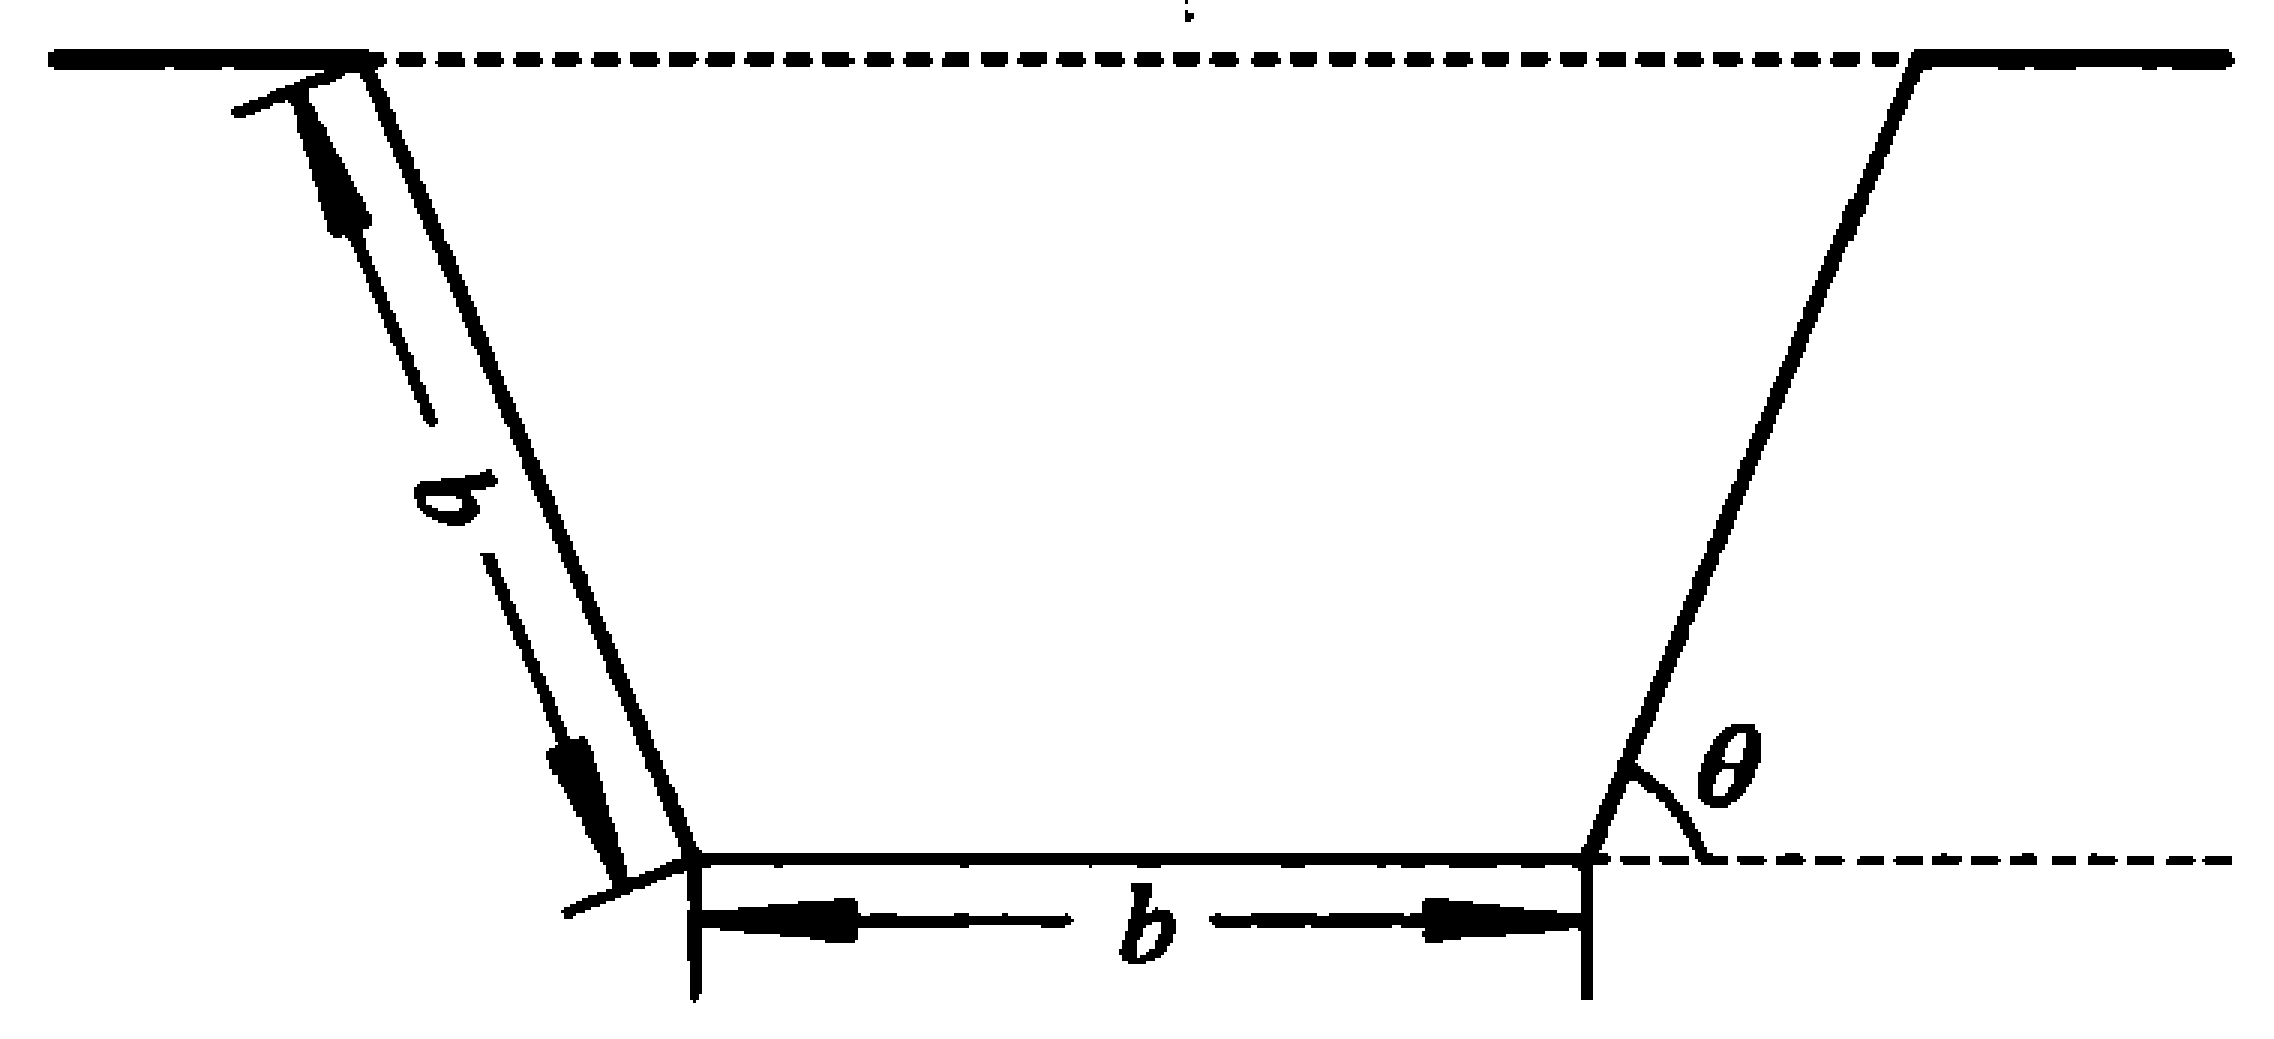
\includegraphics[width=0.4\linewidth]{figures/fig_3_104_1.png}\end{center}
\end{minipage}\par\vfill
\noindent\begin{minipage}{\textwidth}\ProblemHeading{例题}{3.105}
设 $n\in\mathbb N^*$。求 $n+1$ 个多项式 $x^i(1-x)^{n-i}$（$i=0,1,\ldots,n$）在 $[0,1]$ 上的最小值和最大值。
\end{minipage}\par\vfill
\noindent\begin{minipage}{\textwidth}\ProblemHeading{例题}{3.106}
两种均匀介质以平面为分界面，光在两者中的速率分别为 $a,b>0$。点 $A,B$ 分处两侧。根据光程用时最短原则，求从 $A$ 到 $B$ 的光线路径应满足的条件，并解释其与折射角的关系。图中 $\alpha,\beta$ 均为光线与界面的夹角，$A_1,B_1$ 为垂足。
\begin{center}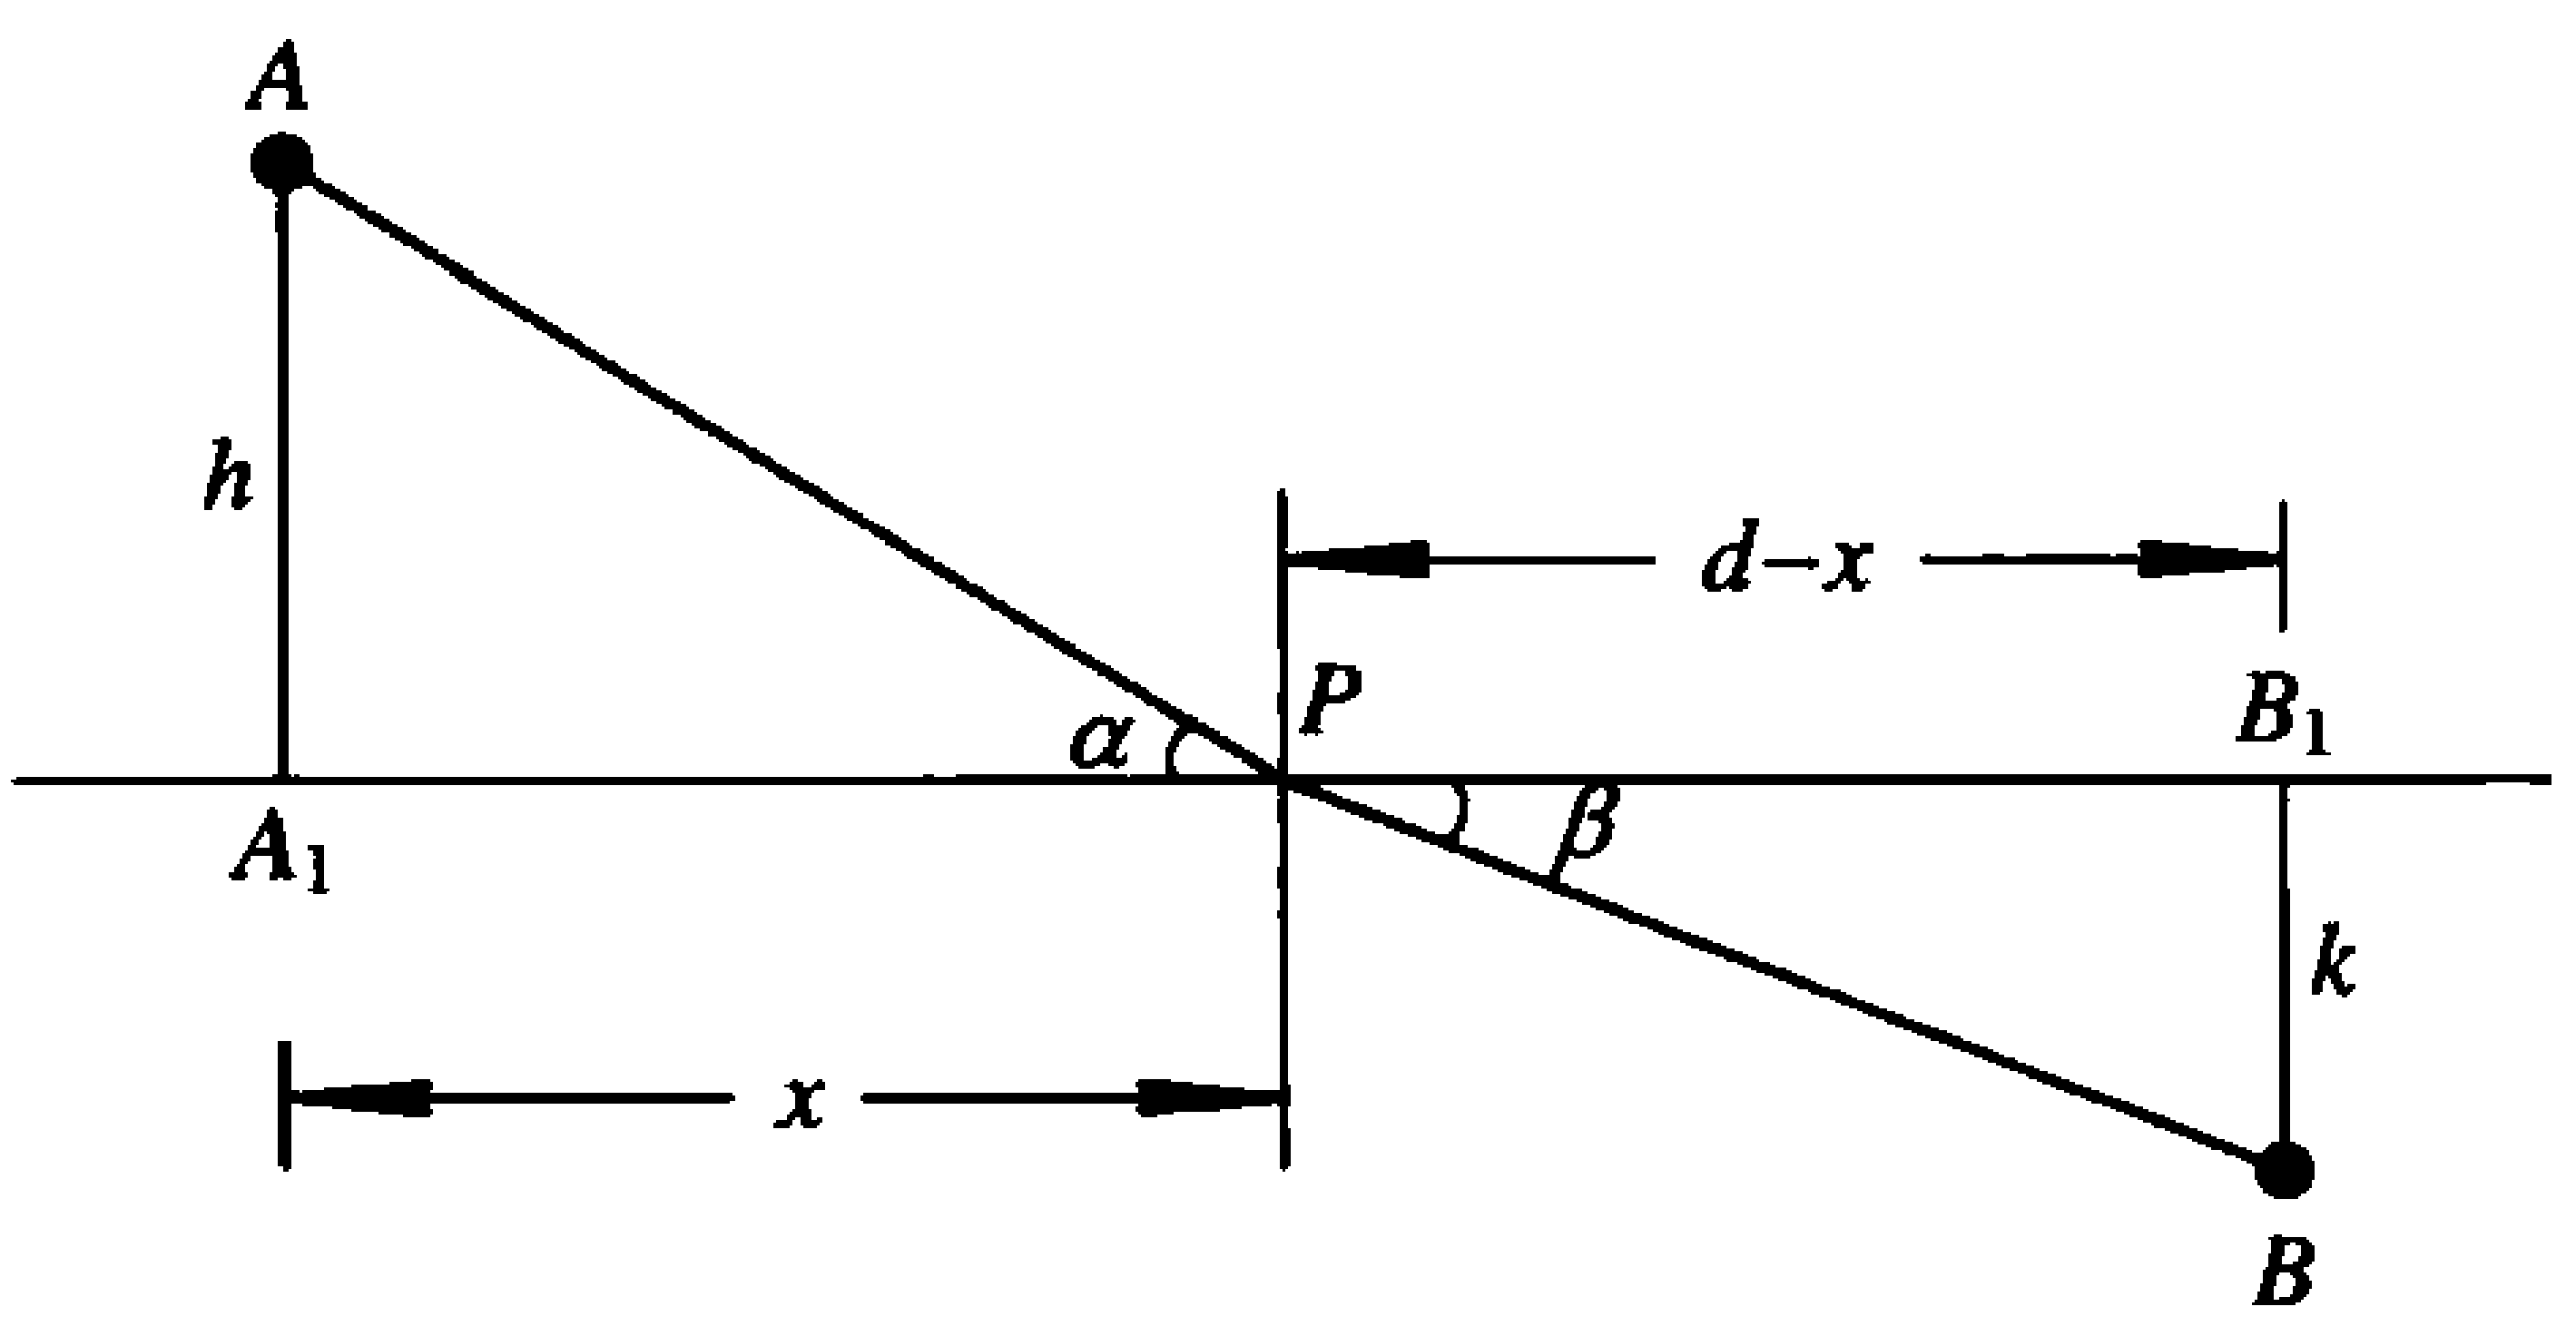
\includegraphics[width=0.42\linewidth]{figures/fig_3_106_1.png}\end{center}
\end{minipage}\par\vfill
\newpage
\noindent\begin{minipage}{\textwidth}\ProblemHeading{例题}{3.107}
设 $a_1,\ldots,a_n$ 为不全相等的正数，定义\[f(x)=\begin{cases}\left(\dfrac{a_1^x+\cdots+a_n^x}{n}\right)^{1/x},&x\ne0,\\(a_1\cdots a_n)^{1/n},&x=0.\end{cases}\]证明 $f$ 在 $\mathbb R$ 上严格递增。
\end{minipage}\par\vfill
\noindent\begin{minipage}{\textwidth}\ProblemHeading{习题}{3.108}
研究下列函数在指定区间内的单调性：
\SubQ{1}{$f(x)=\tan x$，$x\in(-\pi/2,\pi/2)$。}
\SubQ{2}{$f(x)=\arctan x-x$，$x\in\mathbb R$。}
\end{minipage}\par\vfill
\noindent\begin{minipage}{\textwidth}\ProblemHeading{习题}{3.109}
证明下列不等式：
\SubQ{1}{$x(x-\arctan x)>0$，$x\ne0$。}
\SubQ{2}{$x-x^2/2<\ln(1+x)<x$，$x>0$。}
\SubQ{3}{$x-x^3/6<\sin x<x$，$x>0$。}
\end{minipage}\par\vfill
\newpage
\noindent\begin{minipage}{\textwidth}\ProblemHeading{习题}{3.110}
证明下列不等式：
\SubQ{1}{$\ln(1+x)>\dfrac{\arctan x}{1+x}$，$x>0$。}
\end{minipage}\par\vfill
\noindent\begin{minipage}{\textwidth}\ProblemHeading{习题}{3.111}
证明下列不等式：
\SubQ{1}{若 $0<x_1<x_2<\pi/2$，则 $\tan x_2/\tan x_1>x_2/x_1$。}
\SubQ{2}{若 $x,y>0$，$\beta>\alpha>0$，则 $(x^\alpha+y^\alpha)^{1/\alpha}>(x^\beta+y^\beta)^{1/\beta}$。}
\SubQ{3}{若 $x>-1$，则 $(1+x)^\alpha\le1+\alpha x$（$0<\alpha\le1$）；当 $\alpha<0$ 或 $\alpha\ge1$ 时，反向不等式成立。}
\end{minipage}\par\vfill
\noindent\begin{minipage}{\textwidth}\ProblemHeading{习题}{3.112}
证明下列不等式：
\SubQ{1}{若 $p\ge2$，$x\in[0,1]$，则 $((1+x)/2)^p+((1-x)/2)^p\le(1+x^p)/2$。}
\end{minipage}\par\vfill
\newpage
\noindent\begin{minipage}{\textwidth}\ProblemHeading{习题}{3.113}
设 $f$ 在 $[0,1]$ 上有三阶导数，$f(0)=f(1)=0$，令 $F(x)=x^2f(x)$。证明存在 $\xi\in(0,1)$ 使 $F^{\prime\prime\prime}(\xi)=0$。
\end{minipage}\par\vfill
\noindent\begin{minipage}{\textwidth}\ProblemHeading{习题}{3.114}
设 $f$ 在 $[0,+\infty)$ 上可导，$f(0)=0$，且 $f^{\prime}$ 严格递增。证明 $f(x)/x$ 在 $(0,+\infty)$ 上严格递增。
\end{minipage}\par\vfill
\noindent\begin{minipage}{\textwidth}\ProblemHeading{习题}{3.115}
设 $f$ 在 $\mathbb R$ 上有界、二阶可导且 $f^{\prime\prime}\ge0$。证明 $f$ 为常值函数。
\end{minipage}\par\vfill
\newpage
\noindent\begin{minipage}{\textwidth}\ProblemHeading{习题}{3.116}
设 $f,g$ 在 $[a,+\infty)$ 上连续，在 $(a,+\infty)$ 上可导，且 $|f^{\prime}(x)|\le g^{\prime}(x)$。证明对 $x\ge a$ 有 $|f(x)-f(a)|\le g(x)-g(a)$。
\end{minipage}\par\vfill
\noindent\begin{minipage}{\textwidth}\ProblemHeading{习题}{3.117}
证明当 $x>0$ 且 $x\ne1$ 时，有 $(1-x)(x^2\mathrm e^{1/x}-\mathrm e^x)>0$。
\end{minipage}\par\vfill
\noindent\begin{minipage}{\textwidth}\ProblemHeading{习题}{3.118}
求下列函数在指定范围的最大值与最小值；若某一极值不存在，说明理由：
\SubQ{1}{$f(x)=x^4-2x^2+5$，$|x|\le2$。}
\SubQ{2}{$f(x)=\sin(2x)-x$，$|x|\le\pi/2$。}
\SubQ{3}{$f(x)=x\ln x$，$x>0$。}
\end{minipage}\par\vfill
\newpage
\noindent\begin{minipage}{\textwidth}\ProblemHeading{习题}{3.119}
求下列函数在指定范围的最大值与最小值；若某一极值不存在，说明理由：
\SubQ{1}{$f(x)=x^2-3x+2$，$x\in\mathbb R$。}
\SubQ{2}{$f(x)=|x^2-3x+2|$，$|x|\le10$。}
\SubQ{3}{$f(x)=\arctan\dfrac{1-x}{1+x}$，$0\le x\le1$。}
\end{minipage}\par\vfill
\noindent\begin{minipage}{\textwidth}\ProblemHeading{习题}{3.120}
质量为 $W$ 的物体置于粗糙水平面，摩擦系数为 $\mu>0$。对物体施加斜向上的拉力，使它在平面上匀速滑动。拉力应与水平面成何角，才能使所需拉力最小？
\end{minipage}\par\vfill
\noindent\begin{minipage}{\textwidth}\ProblemHeading{习题}{3.121}
内接于椭圆 $x^2/a^2+y^2/b^2=1$（$a,b>0$）且各边平行于坐标轴的矩形，何时面积最大？
\end{minipage}\par\vfill
\newpage
\noindent\begin{minipage}{\textwidth}\ProblemHeading{习题}{3.122}
对于体积一定的圆锥形帐篷（不计底面），其高与底半径之比取何值时，所需篷布面积最小？
\end{minipage}\par\vfill
\noindent\begin{minipage}{\textwidth}\ProblemHeading{习题}{3.123}
从半径为 $R$ 的圆纸片上剪去一个扇形，用余下部分做成圆锥形漏斗。应怎样选择剪去扇形的顶角，才能使漏斗容积最大？
\end{minipage}\par\vfill
\noindent\begin{minipage}{\textwidth}\ProblemHeading{习题}{3.124}
设 $0<a<b\le2a$。在双曲线 $xy=1$ 的横坐标属于 $[a,b]$ 的弧段上作切线。切线与横轴及两条直线 $x=a$、$x=b$ 围成梯形。求使梯形面积最大的切点。
\end{minipage}\par\vfill
\newpage
\noindent\begin{minipage}{\textwidth}\ProblemHeading{习题}{3.125}
对某量作 $n$ 次测量，得到数据 $x_1,\ldots,x_n$。求 $x^*$ 使 $\sum_{i=1}^n(x-x_i)^2$ 在 $x=x^*$ 取得最小值。
\end{minipage}\par\vfill
\noindent\begin{minipage}{\textwidth}\ProblemHeading{习题}{3.126}
求使 $a^x\ge x^a$ 对一切 $x>0$ 成立的所有正数 $a$。
\end{minipage}\par\vfill
\noindent\begin{minipage}{\textwidth}\ProblemHeading{习题}{3.127}
设 $f\in C[a,b]$，在 $(a,b)$ 上可导且 $f^{\prime}$ 单调不减。证明对 $x\in[a,b]$ 有 $(b-x)f(a)+(x-a)f(b)\ge(b-a)f(x)$。
\end{minipage}\par\vfill
\newpage
\noindent\begin{minipage}{\textwidth}\ProblemHeading{习题}{3.128}
判断下列函数在指定定义域内的凸性：
\SubQ{1}{$f(x)=x^\mu$，$\mu\ge1$，$x\ge0$。}
\SubQ{2}{$f(x)=a^x$，$a>0$，$x\in\mathbb R$。}
\SubQ{3}{$f(x)=\ln(1/x)$，$x>0$。}
\end{minipage}\par\vfill
\noindent\begin{minipage}{\textwidth}\ProblemHeading{习题}{3.129}
判断下列函数在指定定义域内的凸性：
\SubQ{1}{$f(x)=x\ln x$，$x>0$。}
\SubQ{2}{$f(x)=-\sin x$，$0\le x<\pi$。}
\end{minipage}\par\vfill
\noindent\begin{minipage}{\textwidth}\ProblemHeading{习题}{3.130}
证明下列不等式，并指出等号成立的条件：
\SubQ{1}{$a^{(x_1+\cdots+x_n)/n}\le(a^{x_1}+\cdots+a^{x_n})/n$，其中 $a>0$、$a\ne1$，$x_i\in\mathbb R$。}
\SubQ{2}{$\dfrac{x_1+\cdots+x_n}{n}\le(x_1^{x_1}\cdots x_n^{x_n})^{1/(x_1+\cdots+x_n)}$，其中 $x_i>0$。}
\SubQ{3}{$x_1^{\lambda_1}\cdots x_n^{\lambda_n}\le\sum_{i=1}^n\lambda_i x_i$，其中 $\lambda_i>0$、$\sum\lambda_i=1$、$x_i\ge0$。}
\end{minipage}\par\vfill
\newpage
\noindent\begin{minipage}{\textwidth}\ProblemHeading{习题}{3.131}
证明同一区间上的两个凸函数之和仍为凸函数。
\end{minipage}\par\vfill
\noindent\begin{minipage}{\textwidth}\ProblemHeading{习题}{3.132}
设 $f:[a,b]\to\mathbb R$ 为凸函数，存在 $c\in(a,b)$ 使 $f(a)=f(c)=f(b)$。证明 $f$ 为常值函数。
\end{minipage}\par\vfill
\noindent\begin{minipage}{\textwidth}\ProblemHeading{习题}{3.133}
设 $a<b<c<d$。若 $f$ 在 $[a,c]$ 和 $[b,d]$ 上均为凸函数，证明 $f$ 在 $[a,d]$ 上也为凸函数。
\end{minipage}\par\vfill
\newpage
\noindent\begin{minipage}{\textwidth}\ProblemHeading{习题}{3.134}
设 $f\in C[a,b]$，在 $(a,b)$ 上二阶可导，$f(a)=f(b)=0$，且存在 $c\in(a,b)$ 使 $f(c)>0$。证明存在 $\xi\in(a,b)$ 使 $f^{\prime\prime}(\xi)<0$。
\end{minipage}\par\vfill
\noindent\begin{minipage}{\textwidth}\ProblemHeading{习题}{3.135}
设 $I$ 为开区间，$f$ 为 $I$ 上的凸函数。证明：
\SubQ{1}{左导函数 $f^{\prime}_-$ 与右导函数 $f^{\prime}_+$ 在 $I$ 上存在且均单调不减，并满足 $f^{\prime}_-(x)\le f^{\prime}_+(x)$。}
\SubQ{2}{若 $f^{\prime}_+$ 在 $x$ 处左连续，或 $f^{\prime}_-$ 在 $x$ 处右连续，则 $f$ 在 $x$ 处可导。}
\SubQ{3}{对每个 $[a,b]\subset I$，存在常数 $M$ 使 $|f(x_2)-f(x_1)|\le M|x_2-x_1|$ 对 $x_1,x_2\in[a,b]$ 成立；由此说明 $f$ 连续。}
\end{minipage}\par\vfill
\noindent\begin{minipage}{\textwidth}\ProblemHeading{习题}{3.136}
设 $I$ 为开区间。证明函数 $f$ 在 $I$ 上为凸函数，当且仅当对每个 $c\in I$，均存在实数 $a$ 使 $f(x)\ge a(x-c)+f(c)$ 对一切 $x\in I$ 成立。作出几何解释。
\end{minipage}\par\vfill
\newpage
\noindent\begin{minipage}{\textwidth}\ProblemHeading{习题}{3.137}
设 $f$ 在区间 $I$ 上可导。证明 $f$ 为凸函数，当且仅当其图像位于每一条切线的上方或线上。
\end{minipage}\par\vfill
\noindent\begin{minipage}{\textwidth}\ProblemHeading{习题}{3.138}
设 $f:[0,+\infty)\to\mathbb R$ 满足 $x=f(x)\mathrm e^{f(x)}$。证明：
\SubQ{1}{$f$ 严格递增。}
\SubQ{2}{$\lim_{x\to+\infty}f(x)=+\infty$。}
\SubQ{3}{$\lim_{x\to+\infty}f(x)/\ln x=1$。}
\end{minipage}\par\vfill
\noindent\begin{minipage}{\textwidth}\ProblemHeading{习题}{3.139}
设多项式 $p$ 满足 $p^{\prime\prime\prime}(x)-p^{\prime\prime}(x)-p^{\prime}(x)+p(x)\ge0$ 对所有实数 $x$ 成立。证明 $p(x)\ge0$。
\end{minipage}\par\vfill
\newpage
\noindent\begin{minipage}{\textwidth}\ProblemHeading{习题}{3.140}
设 $A=(a_{ij})_{n\times n}$ 的所有元素均为正数，每行及每列元素之和均为 $1$。设列向量 $x$ 的分量 $x_1,\ldots,x_n$ 均为正数，$y=Ax$ 的分量为 $y_1,\ldots,y_n$。证明 $y_1\cdots y_n\ge x_1\cdots x_n$。
\end{minipage}\par\vfill
\noindent\begin{minipage}{\textwidth}\ProblemHeading{习题}{3.141}
设边值问题为 $y^{\prime\prime}+p(x)y^{\prime}+q(x)y=r(x)$（$a<x<b$），$y(a)=A$、$y(b)=B$，其中 $q(x)<0$，$A,B$ 为常数。证明：若存在在 $[a,b]$ 上连续、在 $(a,b)$ 上二阶可导的解，则解唯一。
\end{minipage}\par\vfill
\noindent\begin{minipage}{\textwidth}\ProblemHeading{习题}{3.142}
令 $P_n(x)=\sum_{k=0}^n x^k/k!$，$n\in\mathbb N^*$。证明：
\SubQ{1}{当 $x<0$ 时，$P_{2n}(x)>\mathrm e^x>P_{2n+1}(x)$。}
\SubQ{2}{当 $x>0$ 时，$\mathrm e^x>P_n(x)\ge(1+x/n)^n$。}
\end{minipage}\par\vfill
\newpage
\noindent\begin{minipage}{\textwidth}\ProblemHeading{习题}{3.143}
设 $f\in C[a,b]$，且对每个 $x\in(a,b)$，极限 $D^2f(x)=\lim_{h\to0}\dfrac{f(x+h)+f(x-h)-2f(x)}{h^2}$ 存在。若 $D^2f(x)=0$，证明 $f(x)=c_1x+c_2$，其中 $c_1,c_2$ 为常数。
\end{minipage}\par\vfill
\noindent\begin{minipage}{\textwidth}\ProblemHeading{习题}{3.144}
证明对任意正整数 $n$，当 $0<x<\pi$ 时，恒有 $\sum_{k=1}^n\sin(kx)/k>0$。
\end{minipage}\par\vfill
\noindent\begin{minipage}{\textwidth}\ProblemHeading{例题}{3.145}
计算 $\lim_{x\to0}\dfrac{\ln\cos x}{x(x+2)}$。
\end{minipage}\par\vfill
\newpage
\noindent\begin{minipage}{\textwidth}\ProblemHeading{例题}{3.146}
计算 $\lim_{x\to0}\dfrac{x-\sin x}{\sin^3x}$。
\end{minipage}\par\vfill
\noindent\begin{minipage}{\textwidth}\ProblemHeading{例题}{3.147}
设 $f$ 在 $(a,+\infty)$ 上可导，且 $\lim_{x\to+\infty}f^{\prime}(x)=0$。用 L\textquotesingle Hospital 法则证明 $\lim_{x\to+\infty}f(x)/x=0$。
\end{minipage}\par\vfill
\noindent\begin{minipage}{\textwidth}\ProblemHeading{例题}{3.148}
设 $f$ 在 $(a,+\infty)$ 上可导，$\alpha>0$，且 $\lim_{x\to+\infty}(\alpha f(x)+xf^{\prime}(x))=\beta$。证明 $\lim_{x\to+\infty}f(x)=\beta/\alpha$。
\end{minipage}\par\vfill
\newpage
\noindent\begin{minipage}{\textwidth}\ProblemHeading{例题}{3.149}
求 $\lim_{x\to0^+}x^\mu\ln x$，其中 $\mu>0$。
\end{minipage}\par\vfill
\noindent\begin{minipage}{\textwidth}\ProblemHeading{例题}{3.150}
求 $\lim_{x\to\pi/2}(\sec x-\tan x)$。
\end{minipage}\par\vfill
\noindent\begin{minipage}{\textwidth}\ProblemHeading{例题}{3.151}
求 $\lim_{x\to0^+}(\sin x)^x$。
\end{minipage}\par\vfill
\newpage
\noindent\begin{minipage}{\textwidth}\ProblemHeading{例题}{3.152}
求 $\lim_{x\to(\pi/2)^-}(\tan x)^{\pi/2-x}$。
\end{minipage}\par\vfill
\noindent\begin{minipage}{\textwidth}\ProblemHeading{习题}{3.153（校订）}
计算下列极限，出现的参数为常数：
\SubQ{1}{$\lim_{x\to0}\dfrac{\mathrm e^{ax}-\mathrm e^{bx}}{\sin(ax)-\sin(bx)}$，$a\ne b$。}
\SubQ{2}{$\lim_{x\to0}\dfrac{\tan x-x}{x-\sin x}$。}
\SubQ{3}{$\lim_{x\to0}\dfrac{x\cot x-1}{x^2}$。}
\end{minipage}\par\vfill
\noindent\begin{minipage}{\textwidth}\ProblemHeading{习题}{3.154（校订）}
计算下列极限，出现的参数为常数：
\SubQ{1}{$\lim_{x\to0}\dfrac{x(\mathrm e^x+1)-2(\mathrm e^x-1)}{x^3}$。}
\SubQ{2}{$\lim_{x\to+\infty}\dfrac{\mathrm e^x+\mathrm e^{-x}}{x^3}$。}
\SubQ{3}{$\lim_{x\to1^-}\ln x\ln(1-x)$。}
\end{minipage}\par\vfill
\newpage
\noindent\begin{minipage}{\textwidth}\ProblemHeading{习题}{3.155（校订）}
计算下列极限，出现的参数为常数：
\SubQ{1}{$\lim_{x\to0^+}x^x$。}
\SubQ{2}{$\lim_{x\to1}x^{1/(1-x)}$。}
\SubQ{3}{$\lim_{x\to\infty}(\cos(a/x))^x$。}
\end{minipage}\par\vfill
\noindent\begin{minipage}{\textwidth}\ProblemHeading{习题}{3.156（校订）}
计算下列极限，出现的参数为常数：
\SubQ{1}{$\lim_{x\to1}\left(1/\ln x-1/(x-1)\right)$。}
\SubQ{2}{$\lim_{x\to0}\left(1/x-1/(\mathrm e^x-1)\right)$。}
\SubQ{3}{$\lim_{x\to\infty}x\left((1+1/x)^x-\mathrm e\right)$。}
\end{minipage}\par\vfill
\noindent\begin{minipage}{\textwidth}\ProblemHeading{习题}{3.157（校订）}
计算下列极限，出现的参数为常数：
\SubQ{1}{$\lim_{x\to0}\left(\dfrac2\pi\arccos x\right)^{1/x}$。}
\SubQ{2}{$\lim_{x\to+\infty}\left(\dfrac2\pi\arctan x\right)^x$。}
\end{minipage}\par\vfill
\newpage
\noindent\begin{minipage}{\textwidth}\ProblemHeading{习题}{3.158}
设 $f$ 在点 $x$ 处有二阶导数。证明 $f^{\prime\prime}(x)=\lim_{h\to0}\dfrac{f(x+h)+f(x-h)-2f(x)}{h^2}$，并据此推出二阶可导凸函数必满足 $f^{\prime\prime}\ge0$。
\end{minipage}\par\vfill
\noindent\begin{minipage}{\textwidth}\ProblemHeading{习题}{3.159}
设 $f$ 在 $0$ 的某个邻域内有二阶连续导数，且 $f(0)=0$。令 $g(0)=f^{\prime}(0)$，$g(x)=f(x)/x$（$x\ne0$）。证明 $g$ 在此邻域内有连续导函数。
\end{minipage}\par\vfill
\noindent\begin{minipage}{\textwidth}\ProblemHeading{习题}{3.160}
设 $f$ 在 $(a,+\infty)$ 上可导，且 $\lim_{x\to+\infty}\bigl(f(x)+xf^{\prime}(x)\ln x\bigr)=l$。证明 $\lim_{x\to+\infty}f(x)=l$。
\end{minipage}\par\vfill
\newpage
\noindent\begin{minipage}{\textwidth}\ProblemHeading{习题}{3.161}
设 $f$ 在 $(a,+\infty)$ 上有二阶导数，且 $\lim_{x\to+\infty}\bigl(f(x)+2f^{\prime}(x)+f^{\prime\prime}(x)\bigr)=l$。证明 $\lim f(x)=l$、$\lim f^{\prime}(x)=\lim f^{\prime\prime}(x)=0$，这里各极限均取 $x\to+\infty$。
\end{minipage}\par\vfill
\noindent\begin{minipage}{\textwidth}\ProblemHeading{例题}{3.162}
求函数 $y=\dfrac{(1+x)^2}{4(1-x)}$ 的所有渐近线。
\end{minipage}\par\vfill
\noindent\begin{minipage}{\textwidth}\ProblemHeading{例题}{3.163}
作出多项式函数 $f(x)=4x^3-3x$ 的图像。
\end{minipage}\par\vfill
\newpage
\noindent\begin{minipage}{\textwidth}\ProblemHeading{例题}{3.164}
作出函数 $f(x)=(x-1)^2+2\ln x$ 的图像。
\end{minipage}\par\vfill
\noindent\begin{minipage}{\textwidth}\ProblemHeading{例题}{3.165}
作出函数 $y=\dfrac{(1+x)^2}{4(1-x)}$ 的图像。
\end{minipage}\par\vfill
\noindent\begin{minipage}{\textwidth}\ProblemHeading{习题}{3.166}
画出下列曲线，说明定义域、单调性、极值、凹凸性及存在的渐近线：
\SubQ{1}{$y=x^4-2x+10$。}
\SubQ{2}{$y=\mathrm e^{-x^2}$。}
\SubQ{3}{$y=\ln(1+x^2)$。}
\end{minipage}\par\vfill
\newpage
\noindent\begin{minipage}{\textwidth}\ProblemHeading{习题}{3.167}
画出下列曲线，说明定义域、单调性、极值、凹凸性及存在的渐近线：
\SubQ{1}{$y=x-\ln(1+x)$。}
\SubQ{2}{$y=x/(1-x^2)$。}
\SubQ{3}{$y=x^2\mathrm e^{-x}$。}
\end{minipage}\par\vfill
\noindent\begin{minipage}{\textwidth}\ProblemHeading{习题}{3.168}
画出下列曲线，说明定义域、单调性、极值、凹凸性及存在的渐近线：
\SubQ{1}{$y=x/2+\operatorname{arccot}x$，$\operatorname{arccot}$ 取值于 $(0,\pi)$。}
\SubQ{2}{$y=x^4/(1+x)^3$。}
\end{minipage}\par\vfill
